\chapter{Aufbau}

%Bilder vom Aufbau hinzufügen
%Bilder von der Nadelspitze hinzufügen
%Schematische Darstellung von Tunneleffekt und RTM hinzufügen
%Durchführung umstrukturieren und anders einfügen

%add pic stm in general
Das Rastertunnelmikroskop (RTM, engl. STM für Scanning Tunneling Microscope) ist ein hochauflösendes Analyseinstrument zur Darstellung leitfähiger Oberflächen im atomaren Maßstab. Es wurde Anfang der 1980er Jahre von Gerd Binnig und Heinrich Rohrer entwickelt und basiert auf einem fundamentalen quantenmechanischen Phänomen: dem Tunneleffekt.

%add picture tunneleffekt
Dieser Tunneleffekt beschreibt die Möglichkeit von Teilchen, eine Energiebarriere zu durchqueren, obwohl ihre Energie unterhalb der Höhe dieser Barriere liegt. Dies ist ein Verhalten, das aus klassischer Sicht unmöglich wäre. In der Quantenmechanik wird ein Elektron durch eine Wahrscheinlichkeitsverteilung beschrieben, und seine Aufenthaltswahrscheinlichkeit reicht über potenzielle Barrieren hinaus. Wenn sich eine scharf zugespitzte metallische Spitze (in diesem Fall Platinum-Iridium (Pt-Ir)) einer leitfähigen Oberfläche bis auf wenige Ångström nähert und eine geringe Spannung anliegt, besteht eine endliche Wahrscheinlichkeit, dass Elektronen von der Spitze zur Probe oder umgekehrt tunneln. Dieser Tunnelstrom ist extrem empfindlich gegenüber dem Abstand, den er sinkt exponentiell mit wachsender Distanz (d), 
\begin{equation}
    I \propto e^{-\alpha d}, \quad \text{mit } \alpha \approx 1\, \mathrm{\AA}^{-1} %\AA soll Ein Armstrong sein.
\end{equation}
\cite{Tunnelstrom}. Daraus ergibt sich die Möglichkeit, atomare Höhenunterschiede auf der Oberfläche zu detektieren.
%add pic?
Weitere zentrale Begriffe für das Verständnis des STM sind die Austrittsarbeit, jene Mindestenergie, die nötig ist, um ein Elektron aus einem Festkörper ins Vakuum zu bringen, sowie das Ferminiveau, das die höchste besetzte Energieniveaulinie bei absolutem Nullpunkt darstellt. Der Tunnelstrom 
\begin{equation}
    T \propto e^{-2\kappa d}, \quad \text{mit } \kappa = \sqrt{\frac{2m(\Phi - E)}{\hbar^2}}
\end{equation}
\cite{Temperatur}
hängt unter anderem von der Differenz der Ferminiveaus von Spitze und Probe sowie von deren jeweiligen Austrittsarbeiten ab.

\begin{figure}[H]
\centering
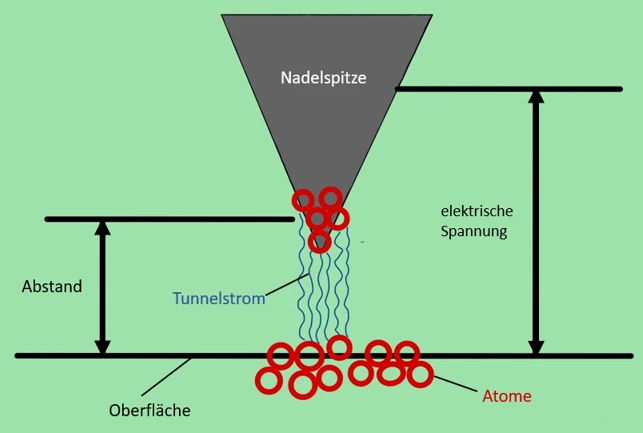
\includegraphics[width=\linewidth]{figs/RTM}
\caption{Aufbau des RTM \cite{RTM}}
\label{fig:RTM}
\end{figure}
Das STM (Abbildung \ref{fig:RTM}) nutzt piezoelektrische Stellglieder zur präzisen Positionierung der Spitze in drei Raumrichtungen. Der dazu entstehende Piezoeffekt beschreibt die Eigenschaft bestimmter Kristalle, sich unter elektrischer Spannung mechanisch zu verformen, in diesem Fall im Sub-Nanometerbereich. Dadurch kann die Spitze rasterartig über die Probe bewegt und gleichzeitig der Abstand hochpräzise geregelt werden. Der Tunnelstrom wird über einen Strom-Spannungswandler detektiert und in einem PID-Regelkreis (Propotional, Integral and Differential) verarbeitet, der die z-Position der Spitze so anpasst, dass der Strom konstant bleibt (constant current mode). Die Spannung am z-Piezo ist damit direkt proportional zur Oberflächenhöhe. Alternativ kann im constant height mode gearbeitet werden, bei dem der Tunnelstrom selbst das Bild liefert, während die Höhe konstant bleibt. Dieser Modus ist schneller, aber risikobehafteter bei rauen Oberflächen.


Es kommen zwei Varianten des STM zum Einsatz: eines mit externem Controller und Easyscan-Software, das andere mit integriertem Controller und NaioSTM-System. Beide Systeme beinhalten ein STM-Gerät, eine Probenhalterung mit Magnetfixierung, eine USB-Lupe zur optischen Kontrolle sowie eine stereoskopische Beobachtungseinheit. Das Gerät wird über einen Computer angesteuert, der auch die Datenaufnahme und Visualisierung übernimmt.

Die STM-Spitze wird durch kontrolliertes Abreißen eines Pt-Ir-Drahts hergestellt und mit einer Halterung in das Gerät eingesetzt. Zur Dokumentation werden sowohl Spitze als auch Probe mit einer USB-Lupe mikroskopiert und kalibriert. Vor Messbeginn wird die Spitze durch mechanisches Advance der Probe angenähert, gefolgt von einem automatisierten Approach, bei dem der Tunnelkontakt präzise erkannt wird.

\chapter{Übersicht des Versuchsablaufs}

%add picture experimentierplatz
%add picture of the box

Die Durchführung des Experiments erfolgt in mehreren Schritten, die im Folgenden detailliert beschrieben werden. Zunächst wird die STM-Spitze vorbereitet und kalibriert, gefolgt von der Probenvorbereitung und der eigentlichen Messung.

Die erste Messungen erfolgt stets im constant current mode, um Schäden an der Spitze durch unkontrollierte Höhenunterschiede zu vermeiden. Typische Startparameter sind eine Tunnelspannung von $U = 1\,\text{V}$ und ein Strom von $I = 1\,\text{nA}$. Die PID-Regelparameter ($P = 1000$, $I = 2000$, $D = 0$) gewährleisten eine stabile Annäherung und Nachführung. Mit der Software wird ein Bildbereich (z.\,B. $200\,\text{nm} \times 200\,\text{nm}$) definiert und gescannt. Die resultierenden Bilder zeigen die topografischen Eigenschaften der Gold-Proben mit hoher lateraler und vertikaler Auflösung.

Zur Analyse von HOPG-Proben wird die Graphitoberfläche zunächst mit Tesafilm abgezogen, um eine frische Schicht freizulegen. Nach dem Einbau wird ein Grobscan durchgeführt. Bei Erfolg werden schrittweise kleinere Bildbereiche gewählt ($10\,\text{nm} \times 10\,\text{nm}$ bis hin zu $4\,\text{nm} \times 4\,\text{nm}$), um atomare Strukturen zu erkennen. Dabei sollten die hexagonale Gitterstruktur von Graphit sichtbar sein. Mit geeigneter Software lassen sich Gitterabstände und -winkel bestimmen, um die Kalibrierung des STM zu überprüfen. Bei Problemen mit der Auflösung helfen Methoden wie Parameteranpassung, Spannungspulse zur Reinigung der Spitze oder der Austausch der Spitze.

Während des gesamten Versuchs werden alle relevanten Messparameter dokumentiert, einschließlich Rastergeschwindigkeit, Spannungs- und Stromwerte, PID-Einstellungen und verwendete Spitze. Die Bilder werden zur Auswertung exportiert und analysiert.
